\documentclass[11pt]{article}
\usepackage[margin=2cm]{geometry}
\usepackage{graphicx}
\usepackage{amsmath}
\usepackage{booktabs}
\usepackage{geometry}
\usepackage{bm}
\usepackage{multicol}
\usepackage{float}
\usepackage{caption}
\usepackage{titlesec}

\usepackage[hypertexnames=false]{hyperref}

\titleformat{\section}{\normalfont\normalsize\bfseries}{\thesection}{1em}{}
\titleformat{\subsection}{\normalfont\normalsize\bfseries}{\thesubsection}{1em}{}

\pagenumbering{gobble}

\geometry{a4paper, margin=2cm}


\title{
	\vspace{-3.5cm}
	\resizebox{\textwidth}{!}{
		Impact Assessment of Windfarm Construction on Animal Density
	}
	\vspace{-2.5cm}
}
\date{}

\begin{document}

\maketitle

\section*{Introduction}
\vspace{-0.35cm}
 This analysis investigates whether the construction of a windfarm affected local bird populations using environmental impact assessment (EIA) data from aircraft bird surveys and data about the proposed construction area. The primary goal is to inform renewable energy stakeholders about potential ecological impacts of windfarm construction, crucial to balancing renewable energy development with ecological preservation. 

\vspace{-0.4cm}
\section*{Methods}
\vspace{-0.35cm}
I choose bird density as our response variable to correct for unequal sampling areas, and square rooted it to ensure the final predicted density (square of response) cannot be negative. Our dataset exhibits spatial and temporal dependencies between covariates which could introduce heteroskedasticity in a non-robust model. I applied exponential weights which allows the model to account for increasing variability in density as predicted values increase. I estimate coefficients using Generalised Least Squares (GLS), which is designed to account for potential heteroskedasticity.

However, even this robust procedure assumes that the residuals are independent and normally distributed after accounting for these specified correlations. This assumption is violated (see \ref{fig:mean_variance}) due to the presence of autocorrelation (see \ref{fig:acf_gls}) caused by uncaptured temporal and spacial variation. I created "blocks" by grouping observations that occurred on the same day to address temporal autocorrelation and within the same grid reference to address spacial autocorrelation. I account for temporal autocorrelation within blocks by incorporating an AR(2) process, where the current observation's error term depends on the errors from the previous two observations within the same block.

To eliminate insignificant covariates, I perform backwards hypothesis testing. Starting with the full model, I remove the single highest p-value predictor and perform an F-test to compare the reduced model against the previous model. This process continues until only statistically significant covariates are left - these were tidestate, observationhour, x.pos, and impact. 

\vspace{-0.4cm}
\section*{Results}
\vspace{-0.35cm}
Windfarm construction had a significant negative impact on bird density ($-11.23\%, p<0.001$). Bird densities were higher during slack tide ($+9.13\%, p<0.001$) and slightly higher during flood tide ($+3.29\%, p=0.031$). Bird sightings decreased as the day progressed ($-2.76\%$ $\text{per hour}, p<0.001$). The significant x.pos term ($p<0.001$) demonstrates that this model does not account for spacial autocorrelation within blocks and is responsible for the remaining ACF in AR(2) (see \ref{fig:acf_gls}).

I used the model to predict density for a given scenario (a slack tide during a July morning at position [1500, 1000]), before and after windfarm construction. Wildlife density fell from 0.55 (95\% confidence interval: 0.47 - 0.64) to 0.42 (95\% confidence interval: 0.35 - 0.49). This decrease in density is unlikely to be due to random variation alone because the before and after confidence intervals do not overlap. 
 
This model exhibits strong non-normality of residuals (see \ref{fig:qq_plot}) and strong heteroskedasticity (see \ref{fig:resid_fitted}). There are a large number of zero bird observations in this dataset (82.59\%). This model fails to account for the inflated zero counts, violating assumptions that the residuals are independent and normally distributed.  

\vspace{-0.4cm}
\section*{Conclusion}
\vspace{-0.35cm}
This model and the resulting predictions suggests that windfarm construction has a significant negative impact on wildlife density, and has significantly decreased during the construction process. 

However, the presence of strong heteroskedasticity and non-normal residuals, largely due to unmodelled inflated zero counts, biases parameter estimates and consequently p-values. This undermined the backwards hypothesis testing process, the conclusion that windfarm construction significantly impacts bird density, and the predictions made using this model. Future researchers could accomodate this inflated zero count to improve parameter estimates by using a zero-inflated Poisson (ZIP) model, where one process models the presence or absence of birds as a Poisson variable and another models the count of birds when they are present.
 
This model succeeds at reducing autocorrelation (see \ref{fig:acf_gls}), with temporal effects removed as insignificant during the hypothesis testing procedure. Further reductions in autocorrelation can be made by employing a spacial autocorrelation model (SAR) to model spacial variance within blocks.


\appendix
\section*{Appendix}

\begin{figure}[H]
    \centering
    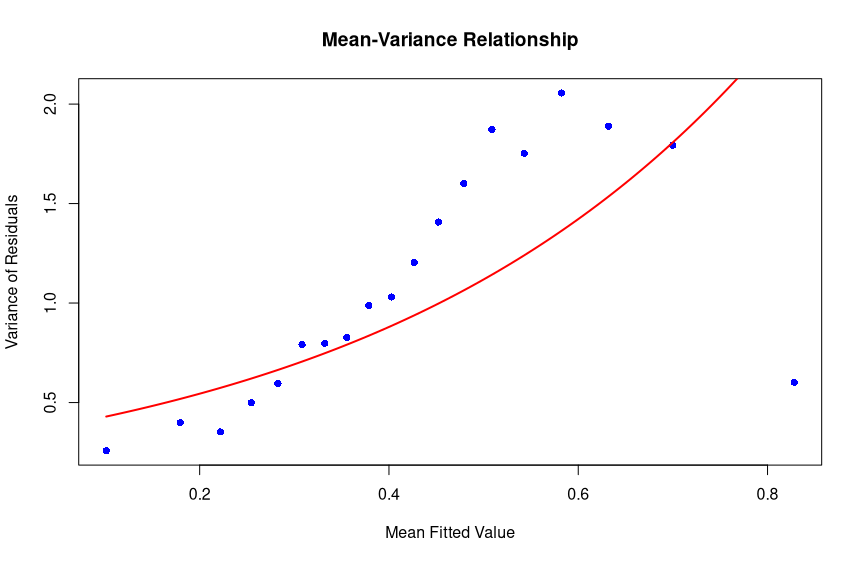
\includegraphics[width=0.7\textwidth]{mean-variance.png}
    \caption{Even the robust model using exponential weights and GLS exhibits significant heteroskedasticity. Residual variance increases non-linearly with the mean fitted value, resulting in the model severely overestimates the variance for the highest predicted root-density values. This pattern indicates that the assumption of normally distributed residuals is violated.}
    \label{fig:mean_variance}
\end{figure}


\begin{figure}[H]
    \centering
    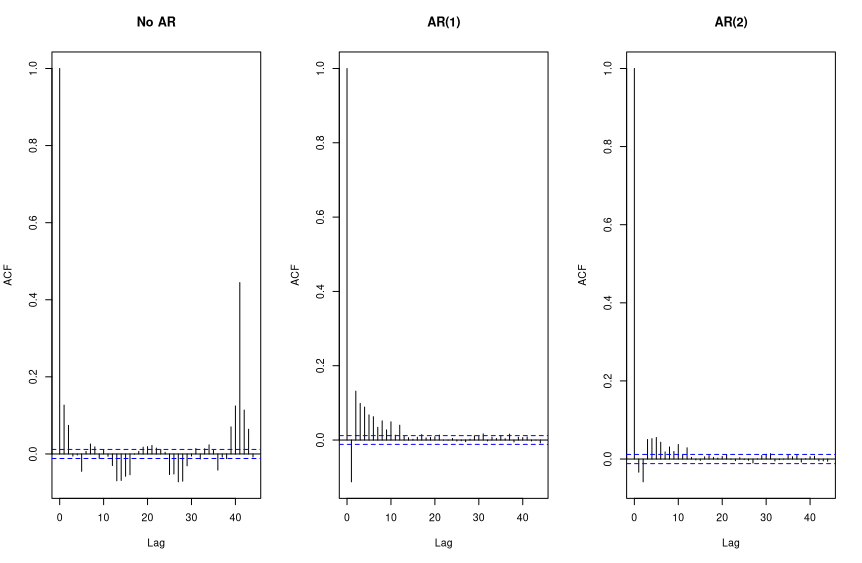
\includegraphics[width=0.8\textwidth]{acf_gls.png}
    \caption{The base model which does not model temporal and spacial dependencies exhibits significant autocorrelation. Introducing blocking and applying an AR(1) structure reduces the residual autocorrelation. By introducing an extra lag, AR(2) reduces the temporal autocorrelation further, but some residual autocorrelation remains especially at low lags.}
    \label{fig:acf_gls}
\end{figure}


\begin{figure}[H]
    \centering
    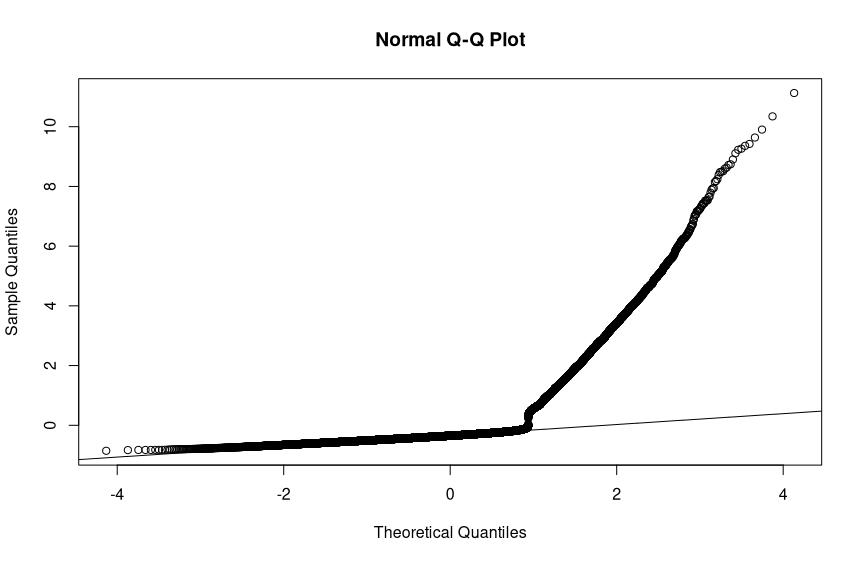
\includegraphics[width=0.7\textwidth]{qq.png}
    \caption{In the reduced AR(2) model, residuals significantly depart from the QQ line at higher sample quantiles, indicating that the assumption of non-normally distributed residuals is violated. This is confirmed by a Shapiro-Wilk test on a random sample of 50 residuals ($p<0.001$).}
    \label{fig:qq_plot} \end{figure}

\begin{figure}[H]
    \centering
    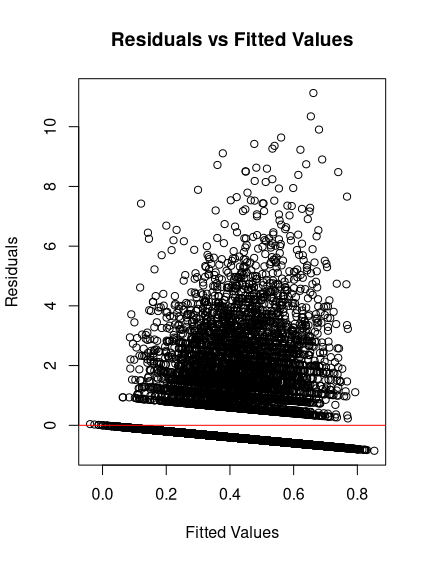
\includegraphics[width=0.5\textwidth]{resid-fitted.png}
    \caption{The residuals of the reduced AR(2) model exhibit funneling, which is indicative of heteroskedasticity. The increasing spread of residuals at higher fitted values suggests that the model's variance is not constant across predictions. This unusual structure is primarily driven by the high number of zero observations in the dataset. Since the model is designed to predict continuous outcomes, the zero values cluster in a line near zero  because the model attempts to fit both the zero and non-zero observations simultaneously. As a result, the model often overpredicts non-zero outcomes, leading to larger residuals as the fitted values increase.}
    \label{fig:resid_fitted}
\end{figure}

\end{document}

